\paragraph*{Evolution in vitro of ribosome activities}
The group of Szostak was also able to develop some in vitro selection systems
that led to the evolution in vitro of ribosome with real enzymatic activity.
After 10 cycles of evolution the activity increased more that 2.5 million fold.

\section{Prokaryotes and Eukaryotes}

Biological organisms can be ``Prokaryotes'' or ``Eukaryotes''. Prokaryotes are
bacteria and archea. They are unicellular organisms with a simple structure,
without internal compartments. Eukaryotes are more complex. Very often they are
multi-cellular organism. They include plants, animals but also many unicellular
organisms (yeast, protozoa and many others). Eukaryotes cells have differents
compartments delimited by internal membranes such as nucleus, mitochondria,
endoplasmic reticulum and Golgi Apparatus.\\

Within \textbf{eukaryotic} cells, DNA is organized into long structures called
\textbf{chromosomes}.
During cell division these chromosomes are duplicated in the process of DNA
replication, providing each cell its own complete set of chromosomes.
Eukaryotic organisms (animals, plants, fungi, and protists) store most of
their DNA inside the cell nucleus and some of their DNA in organelles, such as
mitochondria or chloroplasts.
In contrast, prokaryotes (bacteria and archaea) store their DNA only in the
cytoplasm.
Within the eukaryotic chromosomes, chromatin proteins such as histones compact
and organize DNA.
These compact structures guide the interactions between DNA and other proteins,
helping control which parts of the DNA are transcribed.

During cellular division, the DNA
of Eukaryotes becomes condensed and forms chromosomes that are ``chromo''
because they become easily coloured with basic dyes and are visible under the
microscope.

\paragraph*{Prokaryotes} Prokaryotes are very simple. While the size of a
bacterium is about 1 $\mu$m, a typical Eukaryotic cell is 10-20 times bigger.

Both Prokaryotes and Eukaryotes exchange their genetic information (DNA)
among individuals of the same species. Prokaryotes have a simple system to
transfer some segments of DNA through a ``sex pilus'' from one individual to
another, but they exchange DNA mainly in critical conditions, otherwise they
duplicate as clones.

\subsection{Haploid and diploid}

Definitions

\paragraph*{Diploid}: diploid cells contain two complete sets (2n) of
chromosomes

\paragraph*{Haploid}: haploid cells have half the number of chromosomes (n) as
diploid/they contain only one complete set of chromosomes \\


Be diploid allows you to accumulate faulty genes.

\begin{figure}[H]
  \centering
  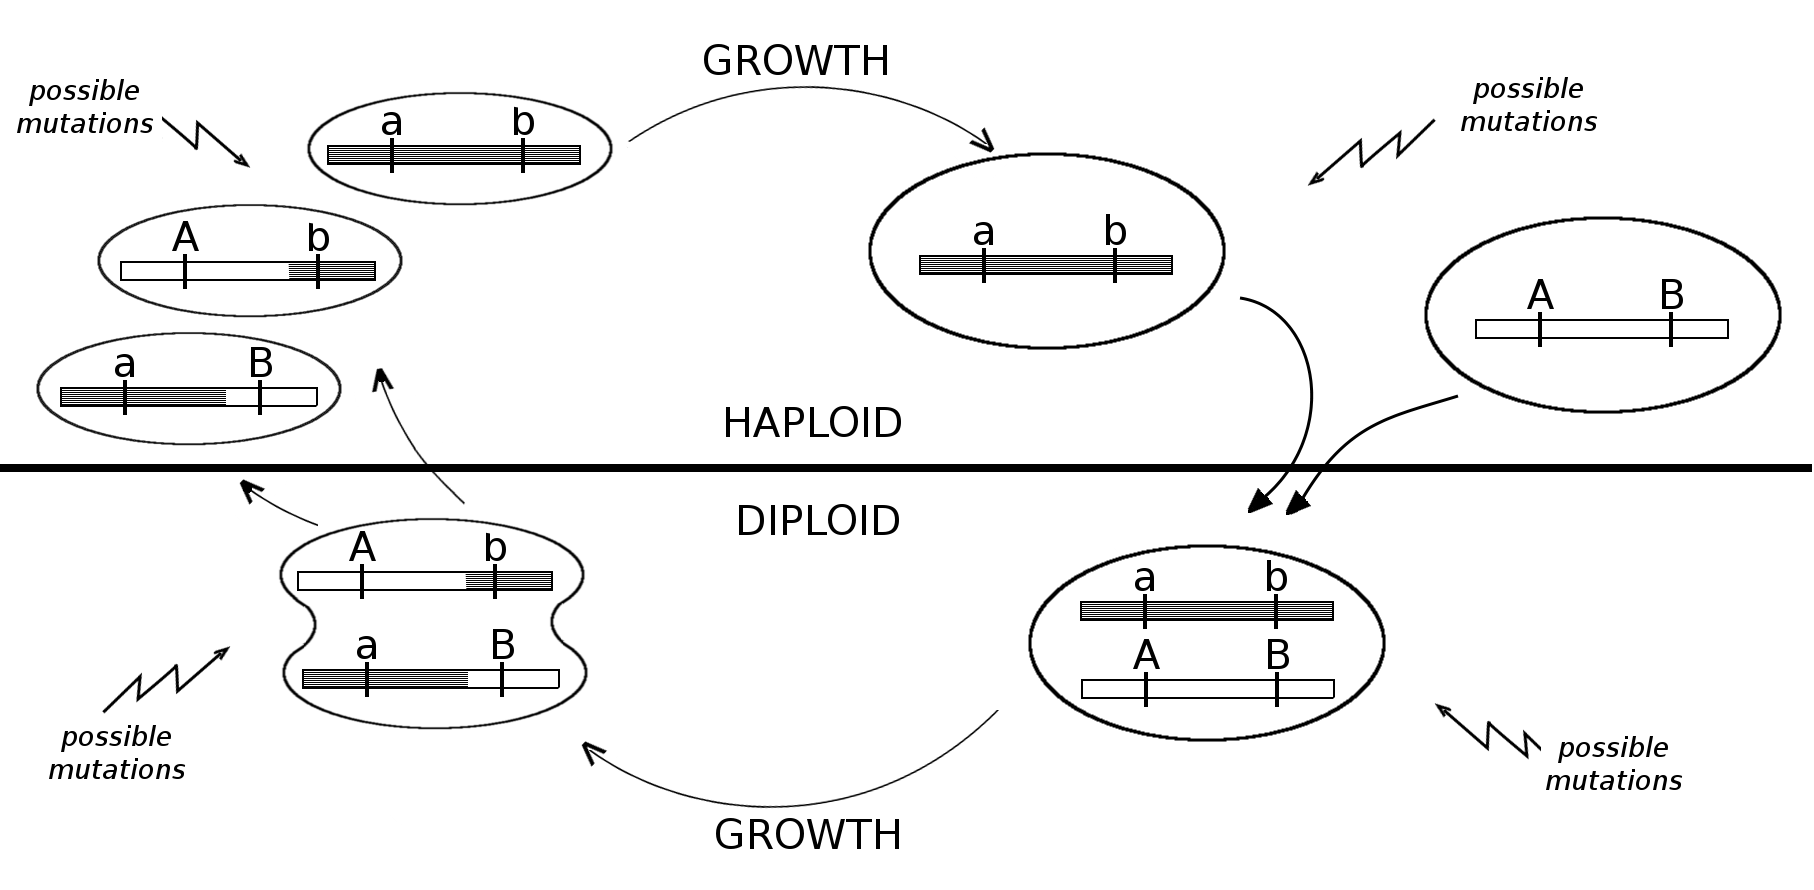
\includegraphics[scale=0.2]{life_cycle}
\end{figure}

During cellular division, the DNA of Eukaryotes becomes condensed and forms
chromosomes. Typically Eukaryotes have sexual reproduction that implies some
alternation between haploid and diploid stages. In Eukaryotes, fertilization
occurs when two haploid cells merge and become one diploid cell. Usually, in a
multi-cellular organism the diploid cells duplicate by \textit{mitosis}; thus a
multi-cellular organism is typically made by many diploid cells with the same
genomics DNA.

\textbf{Meiosis} occurs when a diploid cell produces haploid cells, often
called ``gametes''. During meiosis a process called \textbf{crossing over}
occurs, resulting in the exchange of parts between homologous chromosomes.

In human, the probability that a crossing over occurs within any two loci at
a distance of 1 million bases is about 1\% per generation.
In other organisms may occur with different frequency.

The crossing over, per se, does not produce mutations\footnote{A mutation
happens thanks to an external agent (like radiation) or casually.} but allows
the mix of the genetic diversity present in the two parents. Genetic diversity
is fundamental for evolution. Being diploid allows to maintain a much larger
pool of variant genes, most of these mutated genes do not work as well as the
original, but together with other mutations may improve the fitness.

Some organisms, for instance yeast, have very similar haploid and diploid
cells. Most multi-cellular organisms have a very predominant part of their life
cycle as diploid. The question is: ``Why diploid seems to be better?'' and ``Why
complex organisms (plants and animals) are diploid?''

\paragraph*{Saccharomyces cerevisiae}
First eukaryotic genome that has been sequenced (1996). It's 13 million bases
pairs with 6000 genes.

\paragraph*{Caenorhabditis elegans}
First animal genome that has been sequenced (1998), 100 million base pairs.

\subsection{Cell differentation}

Animals have similar genes, but they are different. The reason behind that is
related to the complexity of an organism, that has the ability to generate many
different type of cells.
Each cell is characterized by a specific set of expressed genes, while the set
nuclear genes remains the same. To create a new cell type with new
characteristics it is not necessary to create new genes but is often sufficient
to change pattern of expression.
